\documentclass[11pt]{article}
\usepackage[spanish]{babel}
\usepackage{float}
\usepackage{graphicx}
\usepackage{geometry}
\geometry{
 a4paper,
 left=15mm,
 top=10mm,
 right=15mm,
 bottom=10mm
 }
\usepackage{hyperref}
\usepackage{lipsum}
\usepackage{tgschola}
\usepackage[T1]{fontenc}
\usepackage{multirow}
\usepackage{amsmath}
\usepackage{fancyhdr}
\usepackage{xcolor}
\usepackage{fontawesome}
\definecolor{modcolour}{gray}{0.6}
\usepackage[none]{hyphenat}
\hypersetup{
   colorlinks=true,
   linkcolor=black,
   urlcolor=blue,
}
\urlstyle{same}
\renewcommand{\contentsname}{Índice}
\setlength{\parskip}{0.5em}

\pagestyle{fancy}

\title{Curriculum Vitae}
\author{Damián Ariel Ponce}

\renewcommand{\headrulewidth}{0pt}
\cfoot{}
% Se actualiza solo yay :D
\rfoot{}

\begin{document}

\noindent
\begin{tabular}[t]{l@{}}
   \hspace{-2mm}\multirow{4}{*}{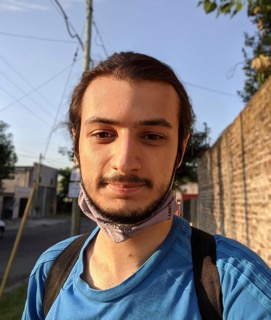
\includegraphics[height=4.5cm]{headshot.jpeg}}
\end{tabular}\hspace{.3cm}
\begin{tabular}[t]{@{}c @{  }l}
   \faMapMarker    & ~Buenos Aires, Argentina                                                      \\[.2cm]
   \faPhone        & ~+54 9 11 3429 0789                                                           \\[.2cm]
   \faEnvelope     & ~\href{mailto:dami.ponce8@gmail.com}{dami.ponce8@gmail.com}                   \\[.2cm]
   \faLinkedin     & ~\href{https://www.linkedin.com/in/damianponce/}{linkedin.com/in/damianponce} \\[.2cm]
   \faGlobe        & ~\href{https://damiponce.github.io/}{damiponce.co}                            \\[.2cm]
   \faBirthdayCake & ~20 years old                                                                 \\

   \\
\end{tabular}
\hfill% move it to the right
\hspace{-2.5cm}
\begin{tabular}[t]{r@{}}
   \\[.2cm]
   \\[.2cm]
   \\[.2cm]
   \\
   \\
   \\
   \textbf{\Huge Damián Ariel Ponce} \\
\end{tabular}

% MAYBE REMOVE \noindent
{\noindent\hrulefill\hspace{-30mm}}

%%%%%%%%%%%%%%%%%%%%%%%%%%%%
\vspace{0.5\baselineskip}\noindent
\renewcommand{\arraystretch}{1}%
\begin{tabular}[t]{@{}p{30mm} @{}p{150mm}}

   %%%%%%%%%%%%%%%%%%%%%%%%%%%%
   {\scshape Education}
                      &
   \textbf{Universidad Tecnológica Nacional (FRH)}  \hfill Haedo, Buenos Aires, Argentina\vspace{0.015in}                                                                       \\ &
   Aeronautical Engineering -- 2nd year \hfill 2021 -- Now\vspace{0.015in}
   \vspace{0.7\baselineskip}
   \\
                      & \textbf{I.N.A.C. C.I.A.T.A.}  \hfill Morón, Buenos Aires, Argentina\vspace{0.015in}                                                                     \\ &
   Secondary school -- Avionics Technician \hfill 2014 -- 2020\vspace{0.015in}
   \\
                      &
   \vspace{.3\baselineskip}
   {\noindent\hspace{-50mm}\hrulefill}
   \vspace{.7\baselineskip}
   \\



   %%%%%%%%%%%%%%%%%%%%%%%%%%%%
   {\scshape Projects}
                      &
   \textbf{Whatsapp Statistics} \href{https://damiponce.github.io/chat-analyser/}{\small(link)}
   \\
   %{\scshape (página web)}
                      &
   Data analysis tool for WhatsApp chats.
   \vspace{0.7\baselineskip}
   \\
                      & \textbf{Web portfolio} \href{https://damiponce.github.io/}{\small(link)}
   \\
                      & A display of my projects and other stuff.
   \vspace{0.7\baselineskip}
   \\
                      & \textbf{Perlin noise 3D Animations} \href{https://damiponce.github.io/3d-noise/}{\small(link)}
   \\
                      & Real-time 3D animations of Perlin noise in the browser.
   \vspace{0.7\baselineskip}
   \\
                      & \textbf{Weather visualization} \href{https://damiponce.github.io/weather-web/}{\small(link)}
   \\
                      & Interactive display for weather data from an open-source API.
   \\
                      &
   \vspace{.3\baselineskip}
   {\noindent\hspace{-50mm}\hrulefill}
   \vspace{.7\baselineskip}
   \\

   %%%%%%%%%%%%%%%%%%%%%%%%%%%%
   {\scshape Abilities}
                      &
   \textbf{Programming languages: }  HTML, CSS, SASS, JavaScript, TypeScript, Python.%, LaTeX, Python.
   \vspace{0.7\baselineskip}
   \\
                      &
   \textbf{Frameworks: }  Node.js, React, React Native.%, LaTeX, Python.
   \vspace{0.7\baselineskip}
   \\
                      &
   \textbf{Tools: }  Git, GitHub, Postman, Photoshop, Illustrator, Figma.%, LaTeX, Python.
   \\
   %\vspace{0.5\baselineskip}
   %&
   %\textbf{Aplicaciones: }  Desarrollo web (front-end), diseño gráfico, edición de %imagenes y documentación.%, dibujo CAD 2D/3D y formateo de texto.
   %\\
                      &
   \vspace{.3\baselineskip}
   {\noindent\hspace{-50mm}\hrulefill}
   \vspace{.7\baselineskip}
   \\
   %  &
   %  \textbf{Software: }  Microsoft Office (Word, Excel, Powerpoint), Photoshop, %  &  Illustrator, Lightroom, AutoCAD, Inventor, Visual Studio Code.
   %  \\
   %  \vspace{1\baselineskip}
   %  \\
   %%%%%%%%%%%%%%%%%%%%%%%%%%%%
   {\scshape Courses} & \textbf{Front-End Web Development with React} \href{https://coursera.org/share/3222a48520eb4c70d96723ded8063968}{\small(link)}  \hfill \vspace{0.015in} \\
                      & Coursera -- The Hong Kong University of Science and Technology \hfill 2022\vspace{0.015in}
   \vspace{0.7\baselineskip}                                                                                                                                                    \\
                      & \textbf{“Radio amateur” (telecommunications) course}  \hfill Morón, Bs.As., Argentina\vspace{0.015in}                                                   \\
                      & I.N.A.C. C.I.A.T.A. \hfill 2018\vspace{0.015in}
   \vspace{0.7\baselineskip}                                                                                                                                                    \\
                      & \textbf{Introductory course to Sensors}  \hfill Morón, Buenos Aires, Argentina\vspace{0.015in}                                                          \\
                      & I.N.A.C. C.I.A.T.A. -- ifm electronics \hfill 2017\vspace{0.015in}                                                                                      \\
                      & \vspace{.3\baselineskip} {\noindent\hspace{-50mm}\hrulefill} \vspace{.7\baselineskip}                                                                   \\
   %%%%%%%%%%%%%%%%%%%%%%%%%%%%
   {\scshape Languages}
                      &
   \textbf{Spanish: }  Native \hspace{3cm} \textbf{English: }  Fluent
   %\vspace{0.7\baselineskip}
   \\
   %&
   %\textbf{Ingles: }  Fluído.
   %\\
                      &
   \vspace{.3\baselineskip}
   {\noindent\hspace{-50mm}\hrulefill}
   \vspace{.7\baselineskip}
   \\

   %%%%%%%%%%%%%%%%%%%%%%%%%%%%
   {\scshape Academic}
                      &
   \textbf{NASA Space Apps Challenge 2019}  \hfill Morón, Buenos Aires, Argentina\vspace{0.015in}                                                                               \\
   {\scshape Experiences} % ???????????
                      & Global nomination for the project\hfill October 2019\vspace{0.015in}
   \vspace{0.7\baselineskip}
   \\
                      & \textbf{Olimpiada Nacional ONIET N$^{\circ}$23}  \hfill Córdoba, Córdoba, Argentina\vspace{0.015in}                                                     \\ &
   4th place at the groups round for Electronics \hfill October 2018\vspace{0.015in}
   \\
                      &
\end{tabular}

\end{document}